\chapter{Requisiti Funzionali}
\label{ch:requisitiFunzionali}

Di seguito vengono riportati i requisiti funzionali (\texttt{RF}) del programma "SatisTrento" tramite \textit{Use Case Diagram} (\texttt{UCD}) progettati usando il linguaggio \texttt{UML}.

% Esempio di markup
\section{\underline{Utente Anonimo}}
    Di seguito i requisiti associati all'Utente Anonimo:
    \begin{itemize}
        \item \textbf{RF1}: Homepage
        \item \textbf{RF2}: Interazione con la mappa
        \item \textbf{RF3}: Multi lingua
        \item \textbf{RF4}: Accesso dati zona selezionata
        \item \textbf{RF5}: Accesso dati specifici zona selezionata
    \end{itemize}
    \begin{figure}[H]
        \centering
        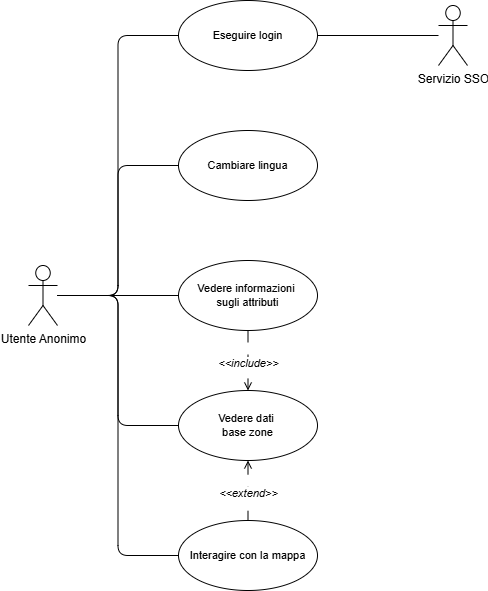
\includegraphics[width=0.8\textwidth]{UseCase_diagrams/Utente_Anonimo.drawio.png}
        \caption{Use Case Diagram dell'Utente anonimo}
    \end{figure}
    \subsection{Use Case {RF1}:Homepage}
        \subsubsection{Riassunto}           % Da discutere quando siamo tutti assieme, ha senso metterlo?
            Questo Use Case descrive come   % Non ha più senso fondere l'RF con un qualche altro RF o qualche parte di un'altro RF?
        \subsubsection{Descrizione}
            Descrizione del requisito uno
        \subsubsection{Eccezioni}
            Ecccezioni del requisito uno
        \subsubsection{Estensioni}
            Estensioni del requisito uno
    \subsection{Use Case {RF2}: Interazione con la mappa}
        \subsubsection{Riassunto}
            Questo Use Case descrive come l'utente potrà interagire con la mappa
        \subsubsection{Descrizione}
            1. L'utente anonimo 
        \subsubsection{Eccezioni}
            1. Se l'utente clicca su di un quartiere già selezionato questo riporterà alla visualizzazione della Homepage
        \subsubsection{Estensioni}
            Estensioni del requisito uno    % Da discutere il concetto dell'estensione per quanto riguarda l'RF2
